% !TEX root = thesis.tex
\chapter{深層学習のアルゴリズム}
Deep Learningは、多層ニューラルネットワークのアイデアをさらに一歩推し進めたもので、学習方法の工夫により、従来よりも多くのレイヤーを扱えて、より複雑な関数を学習できるようになった。数々の分類タスクにて、従来手法を大きくしのぐ成果を収め、注目を浴びている。この章では、Deep Learningがこれまで挙げた成果を紹介すると共に、Deep Learningで使われているアルゴリズムの詳細について述べる。

\section{深層学習の歴史}
多層ニューラルネットワークを学習させるための有用な方法は、まず2006年、Hintonらの研究
Deep Learningの登場 Hinton, Bengio, LeCun
画像認識タスクでの成績、音声認識タスクでの成果、猫認識
MNIST, CIFAR, SVHNなどにおけるconv.net、Maxout, DropConnectの優位

\section{深層学習モデルのバリエーションと詳細}
この節では、Deep Learningのアルゴリズムが、どのような要素の組み合わせで出来ているのか、それぞれの要素はどのようにして学習を助けているのか、紹介する。
\subsection{全体の構造}
(大澤さんのpylearn2の図を一般化したものを書く)
%\subsection{pretraningとfinetuning}
\subsection{ネットワーク構造}
・普通のMLP, SDA, DBM, CNN
\subsection{コスト}
Dropout, DropConnect \\
図\ref{c3_dropconnect}は、DropConnectの著者による紹介Webページ\footnote{\url{http://cs.nyu.edu/~wanli/dropc/}}に掲載されている画像の引用である。ニューラルネットワークにおけるニューロン同士の接続が、ランダムに切断されている様子を表している。
\begin{figure}[tbp]
 \begin{center}
  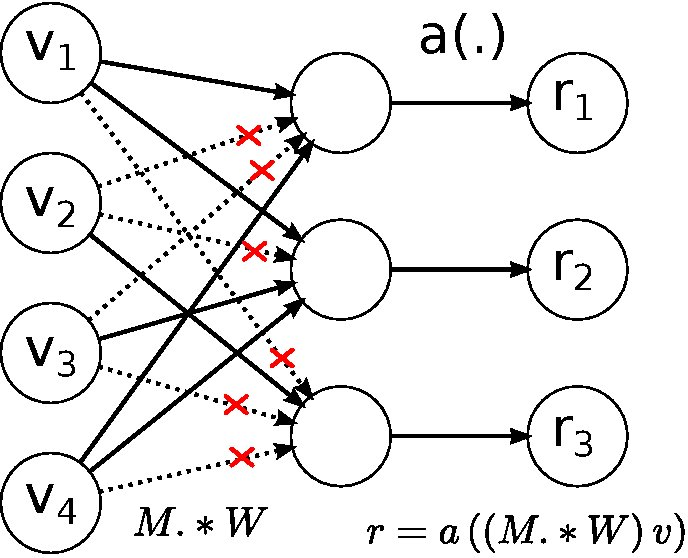
\includegraphics[width=50mm]{img/c3/nn_dc}
 \end{center}
 \caption{DropConnectの模式図}
 \label{c3_dropconnect}
\end{figure}
\subsection{活性化関数}
各ユニットに入力された値は、ある一定の関数によって増幅・変換される。これは人間の神経細胞を真似た仕組みで、神経細胞の化学物質による活性化にちなんで、活性化関数(activation function)と呼ばれる。この項では、Deep Neural Netを構成するときによく用いられる活性化関数を紹介する。
\subsubsection{sigmoidとhyperbolic tangent}
\subsubsection{rectifier}
\subsubsection{Maxout Unit}
線形ユニットの出力を複数まとめて、それらのmaxを取る(=maxout unit)。さらに、複数のmaxout unitの線形和を取ることで、任意の連続関数を近似出来る。\\
図\ref{c3_maxout_app}は、maxout unitが複数の線形ユニットのmaxを取ることによって、様々な凸関数を近似出来る様子を、1次元の入力について示している。
\begin{figure}[tbp]
 \begin{center}
  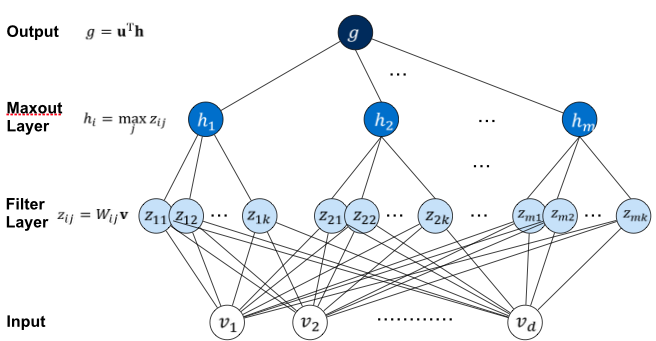
\includegraphics[width=100mm]{img/c3/maxout_arch}
 \end{center}
 \caption{Maxout Networkの構造図}
 \label{c3_maxout_arch}
\end{figure}
\begin{figure}[tbp]
 \begin{center}
  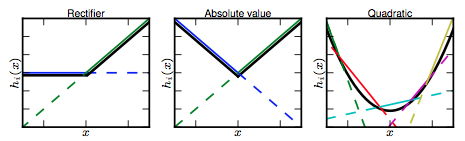
\includegraphics[width=100mm]{img/c3/maxout_app}
 \end{center}
 \caption{Maxout Unitが凸関数を近似する様子(1次元の場合)}
 \label{c3_maxout_app}
\end{figure}
